\documentclass[../Results.tex]{subfiles}

\begin{document}
In this section we present the maps for flux-weighted velocity and flux-weighted dispersion of Ly$\rm \alpha$, HeII and CIV emissions produced with the 3D mask to get an indication of kinematic patterns. We note that Ly$\rm \alpha$ resonant scattering effect doesn't play an important role on kinematics in the central area because it tends to disrupt the coherency of kinematics instead of enhancing it \citep{Cantalupo2005Fluorescent}, this is also confirmed by the results of HeII and CIV emissions.

Fig. \ref{kinematicsmap} shows the moment maps together with the optimally-extracted images of the three emissions. The optimally-extracted images in left panel clearly shows the projected physical scale of Ly$\rm \alpha$ emission extends to 175 kpc which approximates the typical size of dark matter halo at this redshift. This projected scale is smaller comparing to the results of \citet{cai2017discovery} due to small FoV ($\rm 20\arcsec \times 33\arcsec$) of KCWI. In addition, HeII and CIV emission also extends to tens of kpcs surpassing the typical size of galaxies, especially CIV emission which extends to 88 kpc. This spatially very extended metal emissions are rarely seen at high redshift.

In the middle and right panel we present the maps of first and second moment of flux distribution. The middle panel represents the flux-weighted centroid velocity maps, it shows that there are evident velocity gradients in the three velocity maps with same direction from the northwest to the southeast. This kinematic pattern is usually the indication of rotating gas disk in CGM or outflow ejected from central AGN. Besides, the velocity map of Ly$\rm \alpha$ emission also shows gradient around G-5 from northeast to southwest.  The velocity dispersion map of Ly$\rm \alpha$ emission shows that the area around source-B possesses larger velocity dispersion ($\rm \sigma_{v} > 400 \ km/s$) and extends to $\rm \sim 80 \ kpc$. In some spatial positions, dispersion is even larger than 650 km/s which corresponds to FWHM of 1550 km/s. Following the same method in \citet{Arrigoni_Battaia_2018} the expected velocity dispersion calculated for a dark matter halo hosting quasars is $\rm \sim 300 \ km/s$ with the results $\rm M_{DM} \approx 10^{13} \ M_{\odot}$ in \citet{cai2017discovery} where $M_{DM}$ is the mass of dark matter halo. The significant comparison between expected dispersion and our results may indicate that there is extremely powerful kinematic activity in this region which is impossibly caused by rotation or inflow.

Fig. \ref{slices} shows the channel map of Ly$\rm \alpha$ emission with step of 200 km/s. It is clearly seen that the red component and blue component are on either side of source-B. Besides, We also extract the spectra from different spatial positions which are normalized and fitted with one-component gaussian function and show it in Fig. \ref{overlayspec}. We adopt circular aperture with radius of $\rm 1.5 \arcsec$. As a result, the movement of Ly$\rm \alpha$ is clearly seen.

Based on the above analysis, we rule out the possibility that the kinematic pattern is result from rotating gas disk, inflow and resonant scattering effect of Ly$\rm \alpha$ emission. Together with the existing of extended HeII, CIV and OIII emissions \citep{cai2017discovery}, the most natural and straightforward interpretation is that there is extremely powerful and widely influenced outflow ejected from source-B which has the ability to influence the gas environment in dark matter halo hosting source-B. The effect of feedback on large scale has been widely reported before, however these outflows are usually powered by jet with significant radio signal. So, the halo-scale-influenced outflow with no strong radio signal at high redshift makes our observation unique. As a consequence, understanding the mechanism powering this strong outflow in our observation is essential for feedback effect on galaxy evolution.  

	 \begin{figure*}[htp]
		\centering
		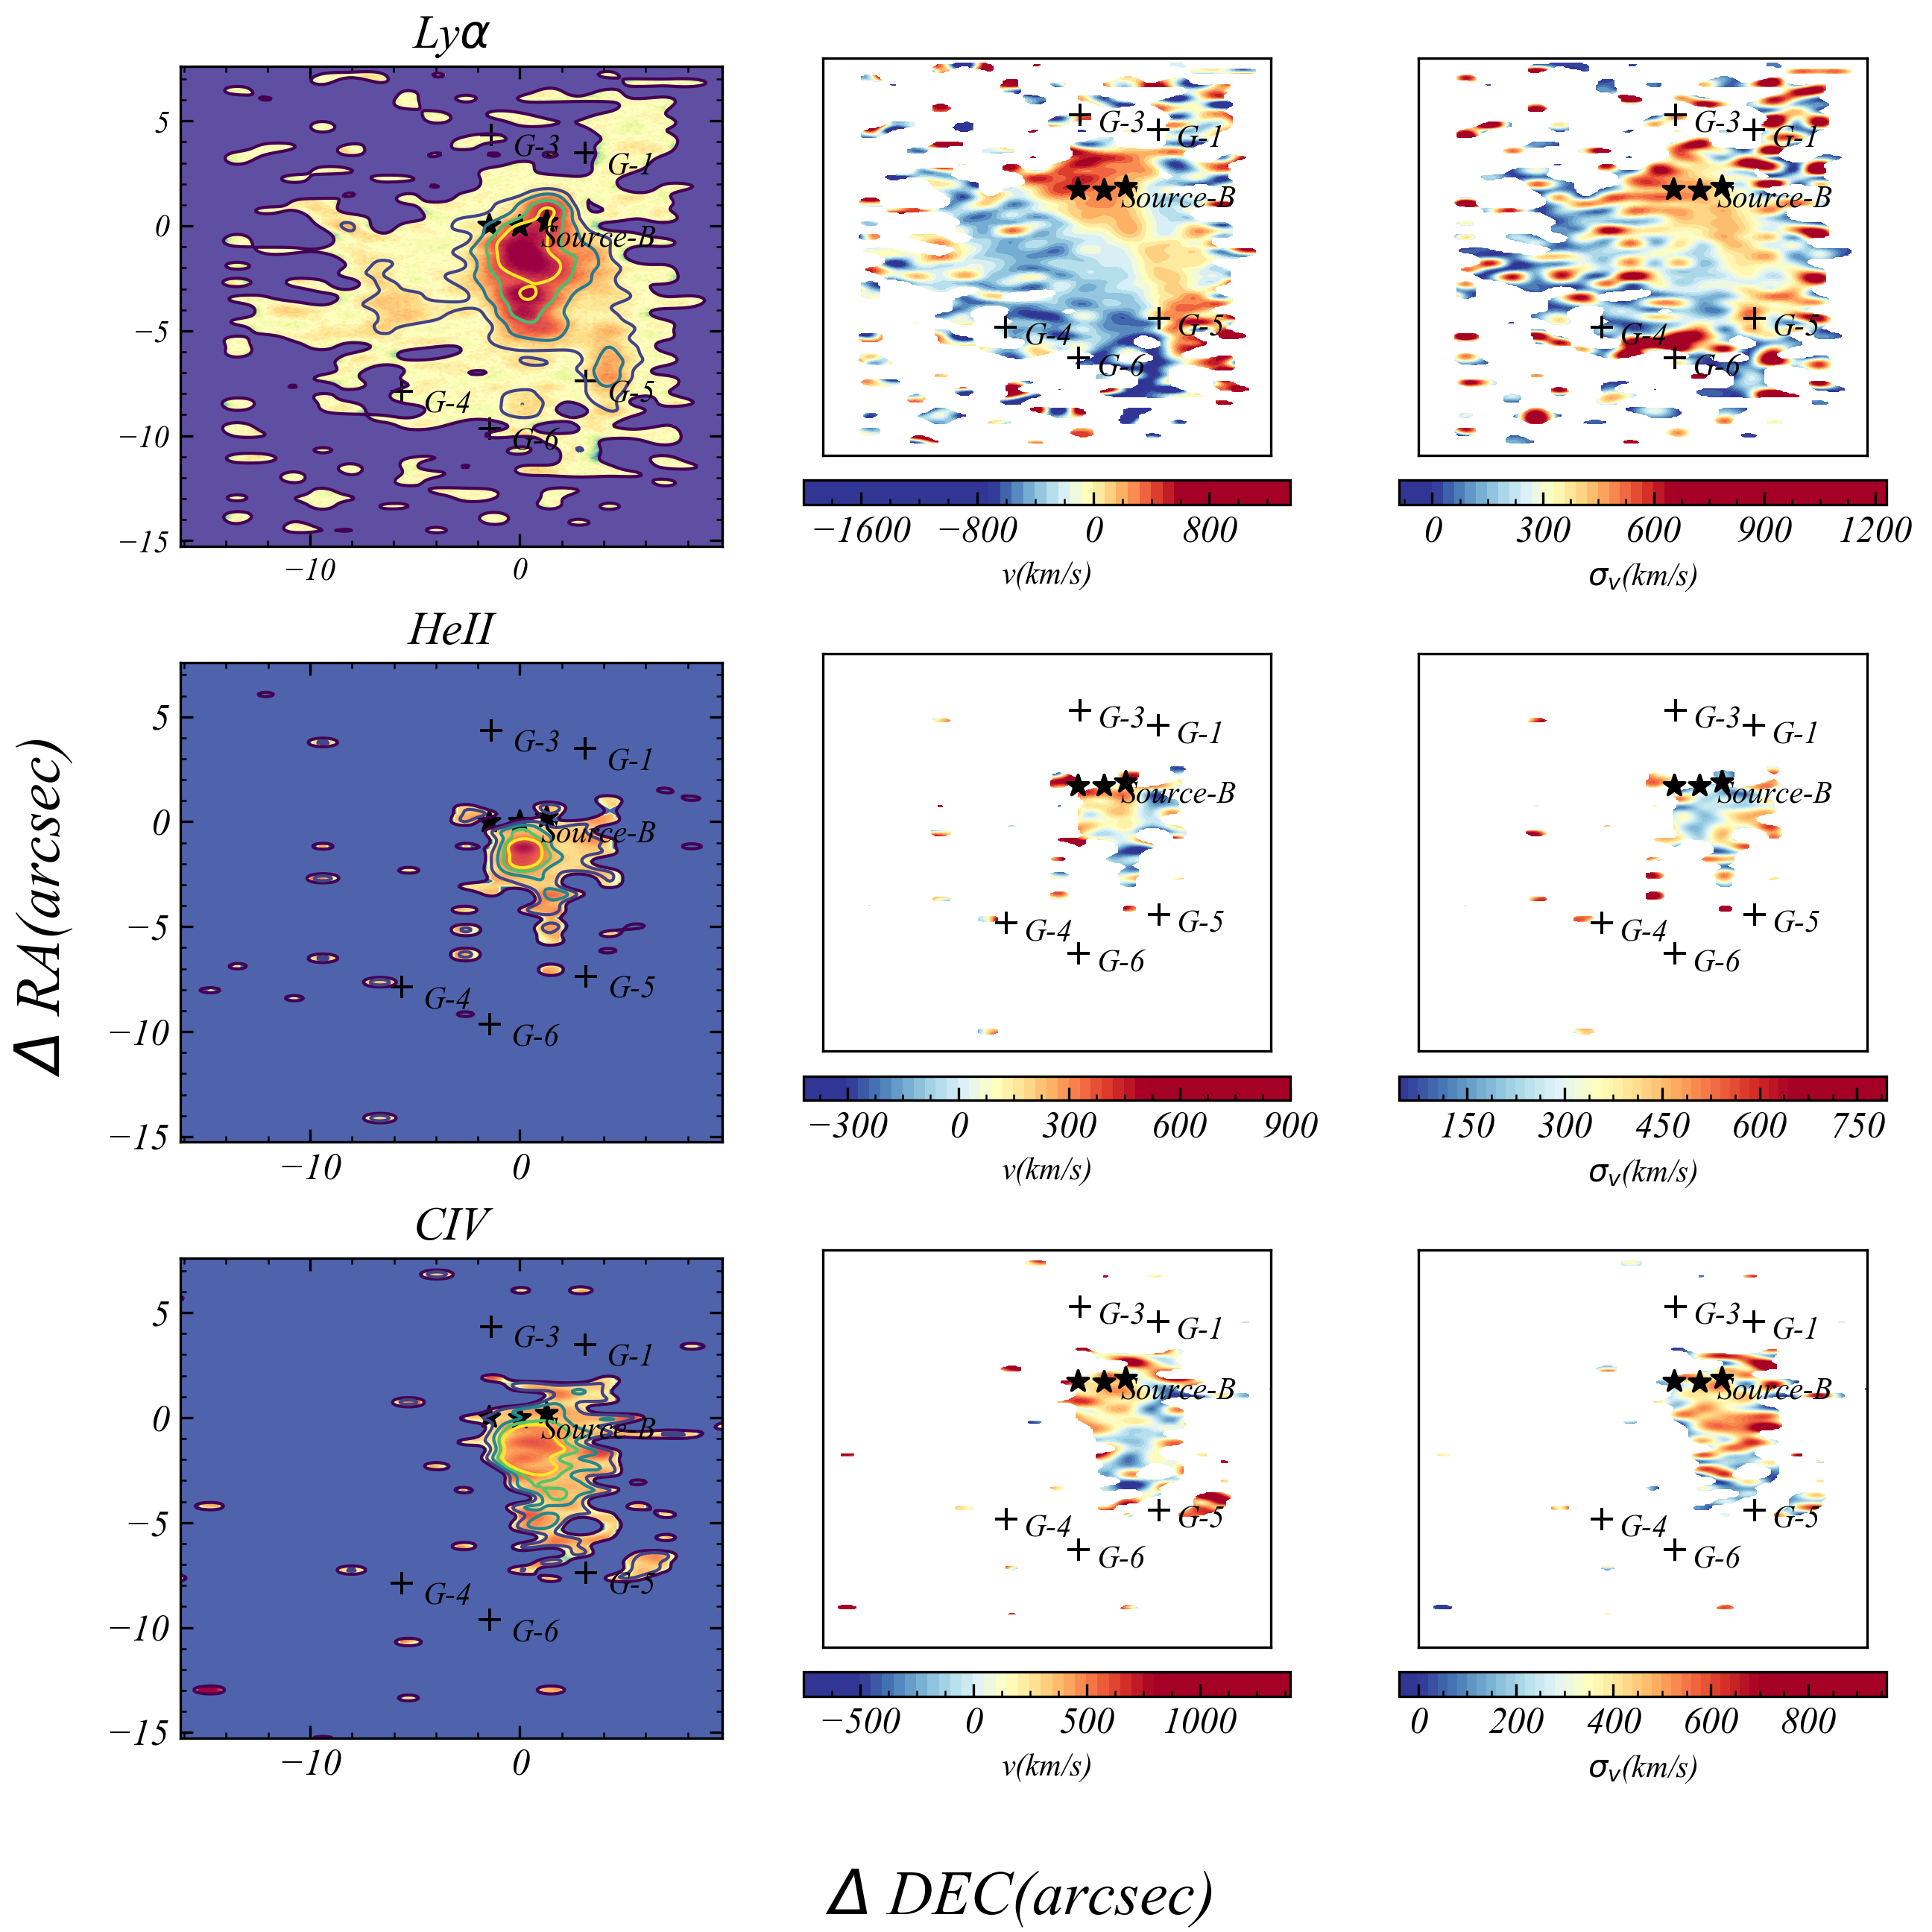
\includegraphics[width=\textwidth]{figs/emissionmap}
		\label{kinematicsmap}
		\caption{Left: continuum-subtracted optimally extracted images for the 3 emissions. Theses images are obtained by stacking each slice together. Pixels with value $\rm < 1.5\sigma$ are masked for each slice. The contour represent signal-to-noise ratio(SNR). We adopt ($\rm 5\sigma,9\sigma,18\sigma,30\sigma,42\sigma,51\sigma$), ($\rm 3\sigma,5,9\sigma$) and ($\rm 4\sigma,7\sigma,9\sigma$) for Ly$\rm \alpha$, HeII and CIV respectively. Middle: flux-weighted velocity map obtained from the first-moment of flux distribution with respect to the systemic redshift of MAMMOTH-1. Right: flux-weighted velocity dispersion obtained from the second-moment of the flux distribution. Sources at the same redshift with MAMMOTH-1 confirmed by CO (2-1) emission \citep{emonts2019cold} and CO (3-2) emission \citep{qiongli2020} are also marked. }
	\end{figure*}
	
	\begin{figure*}[htp]
		\centering
		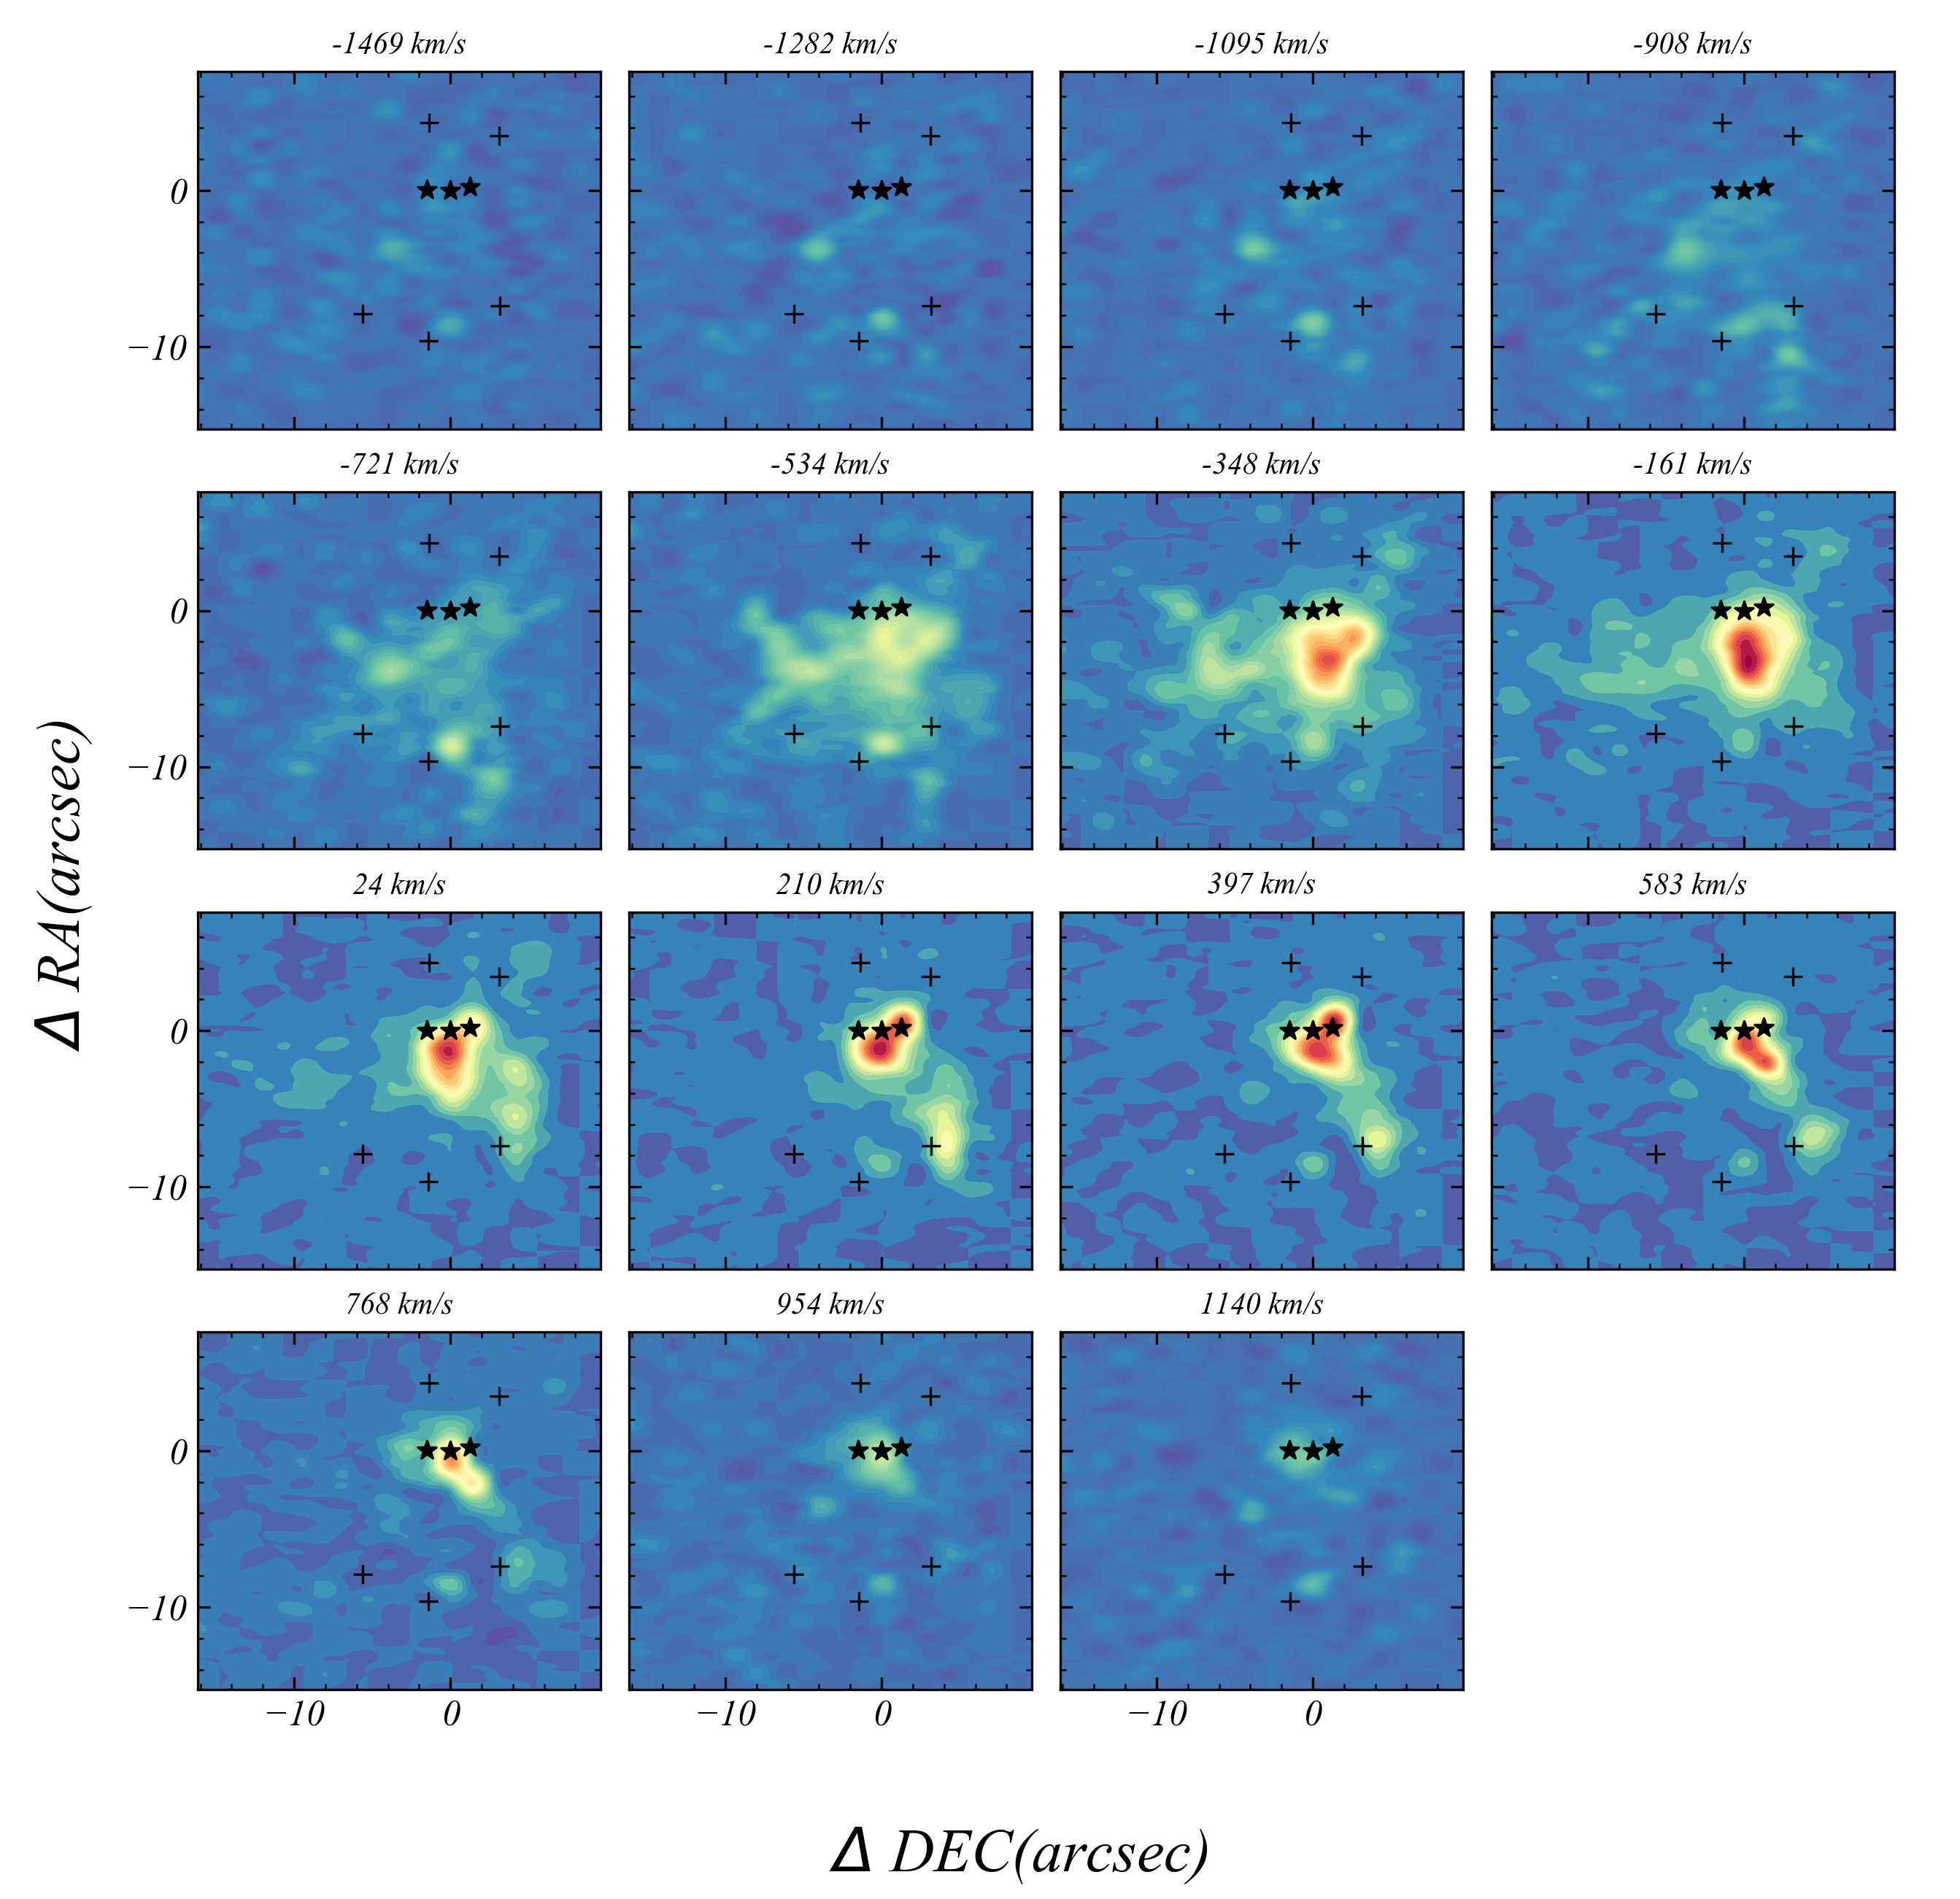
\includegraphics[width=\textwidth]{figs/slices}
		\label{slices}
		\caption{Channel maps for Ly$\rm \alpha$ emission in the wavelength coverage of 4000-4040 \AA. We adopt $\rm \Delta v= 187 \ km/s$ which corresponds to 4 \AA$^{-1}$ as the bin size. It shows fully separated red and blue components on either side of source-B which are the evidences of outflow.}
	\end{figure*}
	
	\begin{figure*}[htp]
		\centering
		\subfloat[Map]{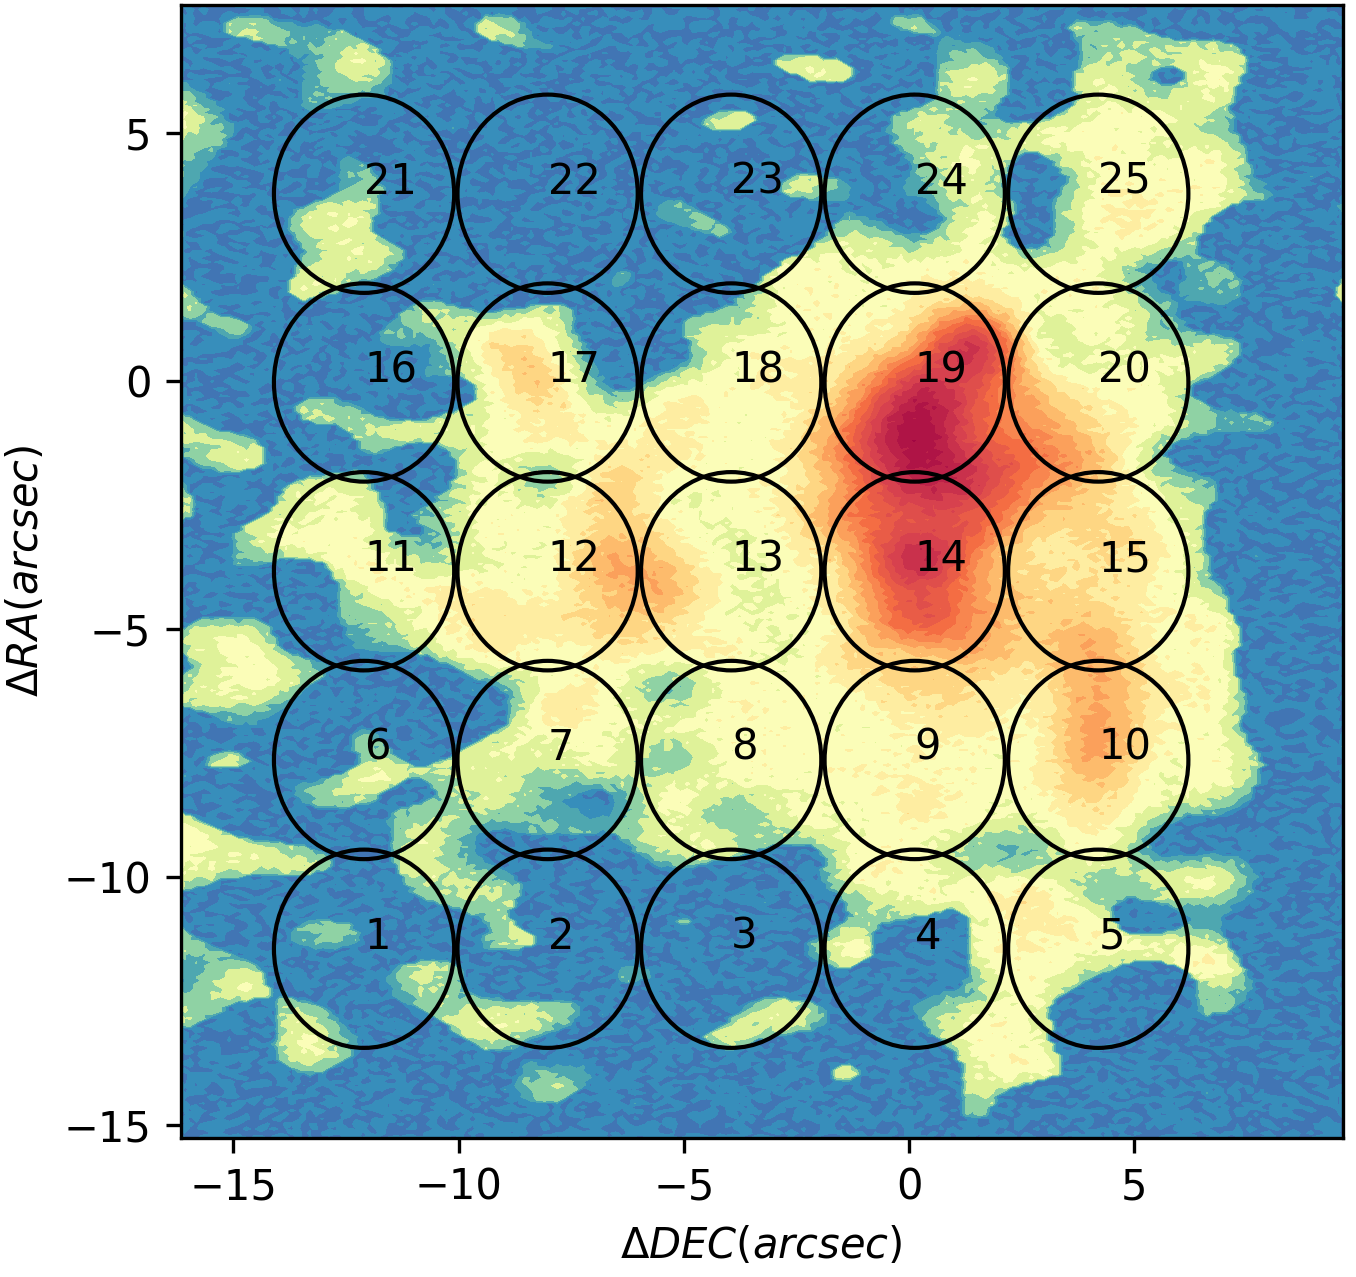
\includegraphics[width=0.5\textwidth]{figs/apertmap.png}}
		\subfloat[Spectra]{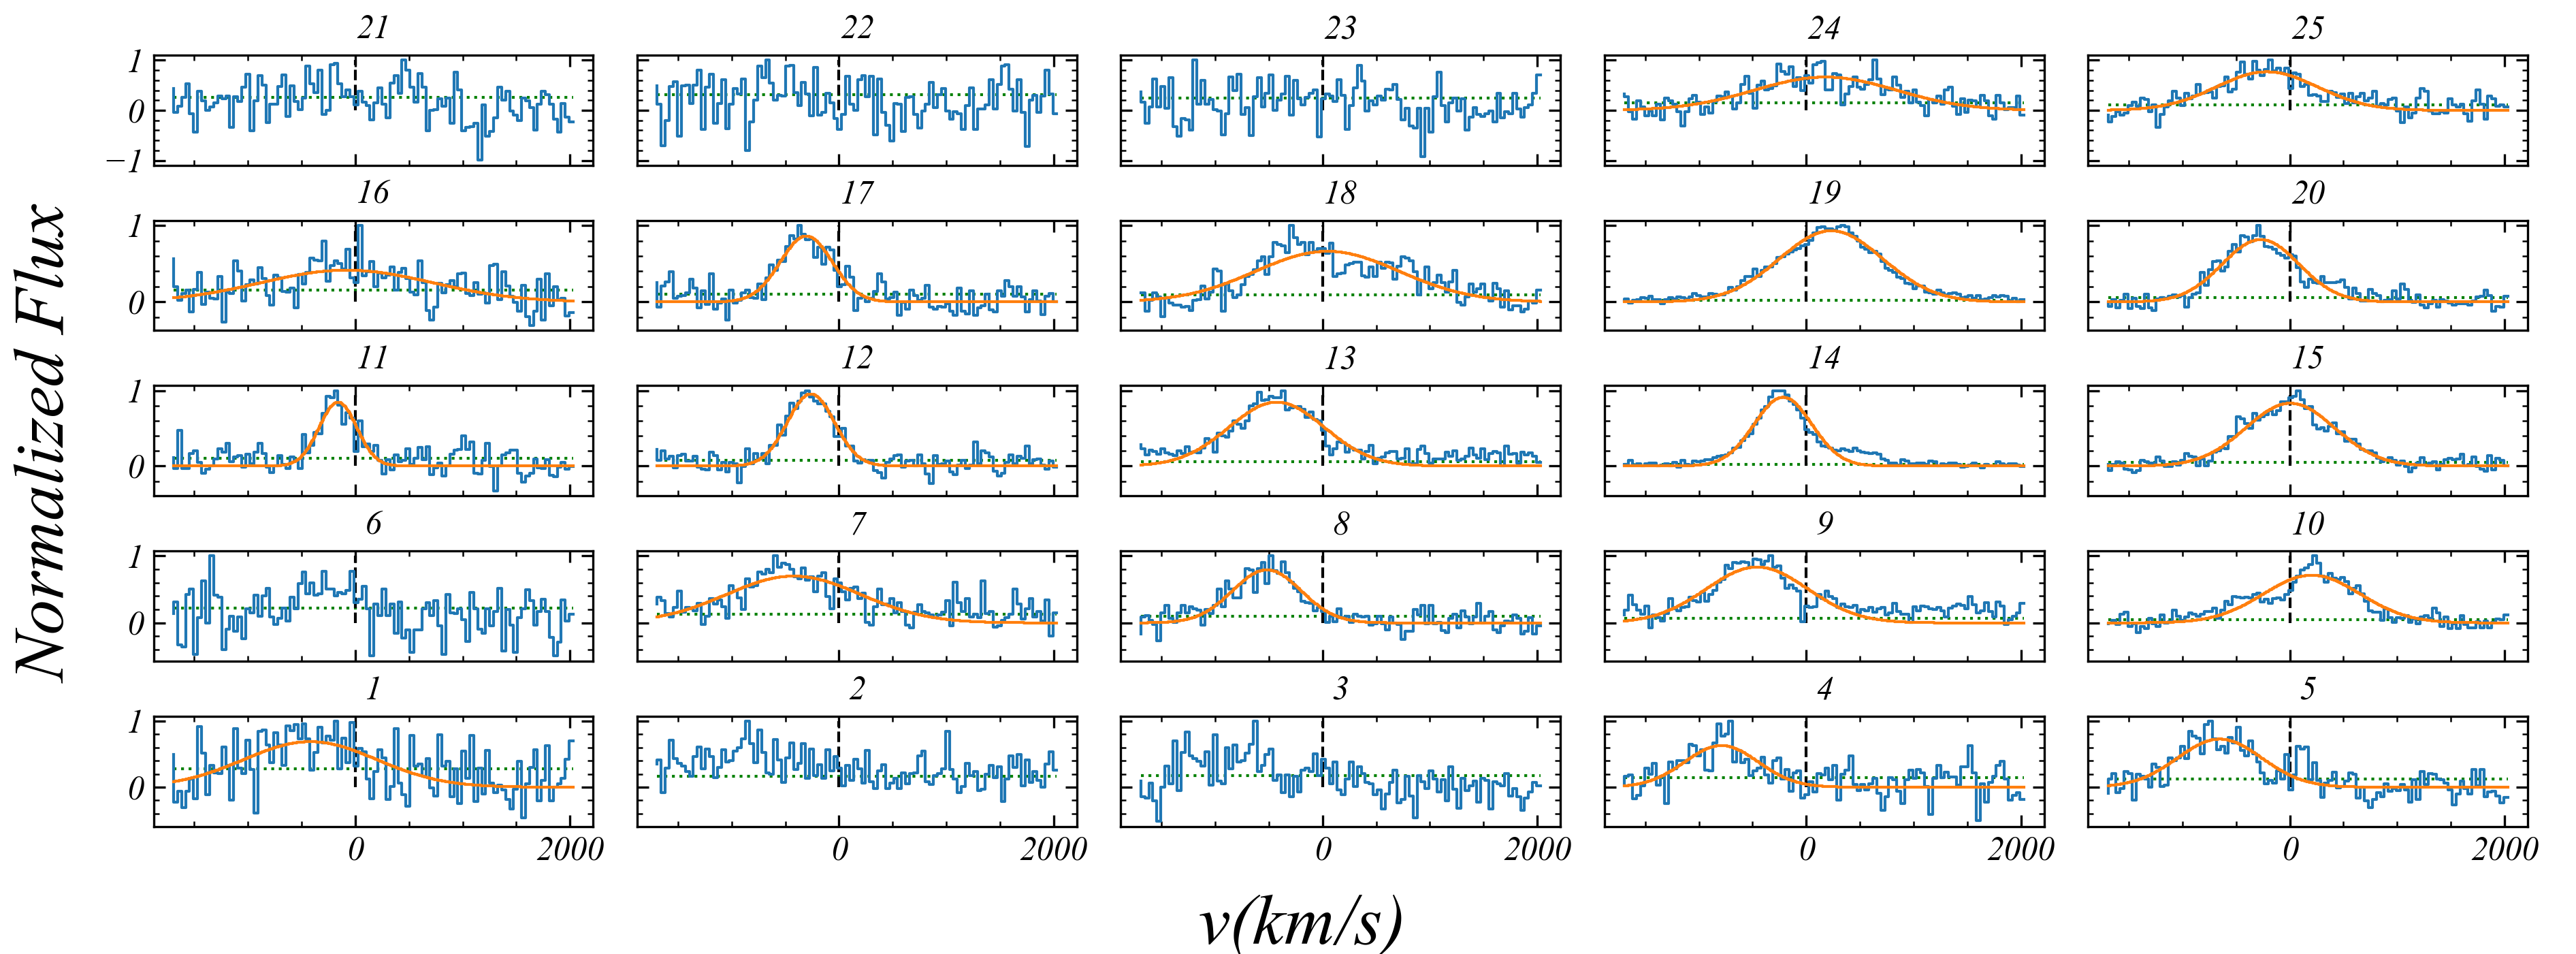
\includegraphics[width=0.5\textwidth]{figs/specmap}}
		\label{overlayspec}
		\caption{Left: Optimally extracted image of Ly$\rm \alpha$ emission. The circular apertures and numbers indicate the spatial regions from which we extracted the spectra shown in the right panel. Right: continuum-subtracted spectra extracted from the individual spatial regions indicated in the left panel. The gray vertical lines represent the location of $\rm v=0 \ km/s$, the green lines represent the noise level for each spectrum and the orange lines represent the fitting results of the Ly$\rm \alpha$ emission for different spatial positions. The flux has been normalized.}
	\end{figure*}
\begin{center}
\begin{table*}[htp]
\begin{tabular}{llllllllllllllllllll}
\hline
\hline
Number & 1    & 4    & 5    & 7    & 8    & 9    & 10   & 11   & 12   & 13   & 14   & 15  & 16   & 17   & 18   & 19   & 20   & 24   & 25   \\
\hline
Velocity(km/s)   & -416 & -785 & -649 & -419 & -515 & -453 & 208  & -157 & -257 & -424 & -211 & 9    & -75  & -300 & 49   & 236  & -267 & 182  & -208 \\
Dispersion(km/s) & 618  & 342  & 392  & 626  & 319  & 474  & 450  & 174  & 219  & 444  & 269  & 415  & 799  & 242  & 668  & 481  & 358  & 660  & 472  \\
$f_{norm}$       & 0.69 & 0.63 & 0.73 & 0.70 & 0.79 & 0.83 & 0.71 & 0.84 & 0.95 & 0.85 & 0.91 & 0.83 & 0.41 & 0.86 & 0.66 & 0.93 & 0.81 & 0.66 & 0.77 \\
\hline
\end{tabular}
\label{fitpara}
\end{table*}
\end{center}
	
\end{document}